\documentclass[]{book}
\usepackage{lmodern}
\usepackage{amssymb,amsmath}
\usepackage{ifxetex,ifluatex}
\usepackage{fixltx2e} % provides \textsubscript
\ifnum 0\ifxetex 1\fi\ifluatex 1\fi=0 % if pdftex
  \usepackage[T1]{fontenc}
  \usepackage[utf8]{inputenc}
\else % if luatex or xelatex
  \ifxetex
    \usepackage{mathspec}
  \else
    \usepackage{fontspec}
  \fi
  \defaultfontfeatures{Ligatures=TeX,Scale=MatchLowercase}
\fi
% use upquote if available, for straight quotes in verbatim environments
\IfFileExists{upquote.sty}{\usepackage{upquote}}{}
% use microtype if available
\IfFileExists{microtype.sty}{%
\usepackage{microtype}
\UseMicrotypeSet[protrusion]{basicmath} % disable protrusion for tt fonts
}{}
\usepackage[margin=1in]{geometry}
\usepackage{hyperref}
\hypersetup{unicode=true,
            pdftitle={Big Questions and Probabilistic Answers},
            pdfauthor={Yoav Bergner},
            pdfborder={0 0 0},
            breaklinks=true}
\urlstyle{same}  % don't use monospace font for urls
\usepackage{natbib}
\bibliographystyle{apalike}
\usepackage{longtable,booktabs}
\usepackage{graphicx,grffile}
\makeatletter
\def\maxwidth{\ifdim\Gin@nat@width>\linewidth\linewidth\else\Gin@nat@width\fi}
\def\maxheight{\ifdim\Gin@nat@height>\textheight\textheight\else\Gin@nat@height\fi}
\makeatother
% Scale images if necessary, so that they will not overflow the page
% margins by default, and it is still possible to overwrite the defaults
% using explicit options in \includegraphics[width, height, ...]{}
\setkeys{Gin}{width=\maxwidth,height=\maxheight,keepaspectratio}
\usepackage[normalem]{ulem}
% avoid problems with \sout in headers with hyperref:
\pdfstringdefDisableCommands{\renewcommand{\sout}{}}
\IfFileExists{parskip.sty}{%
\usepackage{parskip}
}{% else
\setlength{\parindent}{0pt}
\setlength{\parskip}{6pt plus 2pt minus 1pt}
}
\setlength{\emergencystretch}{3em}  % prevent overfull lines
\providecommand{\tightlist}{%
  \setlength{\itemsep}{0pt}\setlength{\parskip}{0pt}}
\setcounter{secnumdepth}{5}
% Redefines (sub)paragraphs to behave more like sections
\ifx\paragraph\undefined\else
\let\oldparagraph\paragraph
\renewcommand{\paragraph}[1]{\oldparagraph{#1}\mbox{}}
\fi
\ifx\subparagraph\undefined\else
\let\oldsubparagraph\subparagraph
\renewcommand{\subparagraph}[1]{\oldsubparagraph{#1}\mbox{}}
\fi

%%% Use protect on footnotes to avoid problems with footnotes in titles
\let\rmarkdownfootnote\footnote%
\def\footnote{\protect\rmarkdownfootnote}

%%% Change title format to be more compact
\usepackage{titling}

% Create subtitle command for use in maketitle
\providecommand{\subtitle}[1]{
  \posttitle{
    \begin{center}\large#1\end{center}
    }
}

\setlength{\droptitle}{-2em}

  \title{Big Questions and Probabilistic Answers}
    \pretitle{\vspace{\droptitle}\centering\huge}
  \posttitle{\par}
  \subtitle{Data Science You Can Use for Stuff You Care About}
  \author{Yoav Bergner}
    \preauthor{\centering\large\emph}
  \postauthor{\par}
      \predate{\centering\large\emph}
  \postdate{\par}
    \date{2019-05-24}

\usepackage{booktabs}
\usepackage{amsthm}
\makeatletter
\def\thm@space@setup{%
  \thm@preskip=8pt plus 2pt minus 4pt
  \thm@postskip=\thm@preskip
}
\makeatother

\begin{document}
\maketitle

{
\setcounter{tocdepth}{1}
\tableofcontents
}
\hypertarget{preface}{%
\chapter*{Preface}\label{preface}}
\addcontentsline{toc}{chapter}{Preface}

\begin{quote}
``\ldots{}the most important questions of life, which are for the most part only problems of probability. It may even be said, strictly speaking, that almost all our knowledge is only probabilistic.''

--- Pierre Simon, Marquis de Laplace
\end{quote}

This book is an incomplete draft of a work in progress being developed as lecture notes for an online course. Content is provisional, contingent, and possibly wrong, but always well intended.

\hypertarget{guiding-principles-in-this-book}{%
\section*{Guiding principles in this book}\label{guiding-principles-in-this-book}}
\addcontentsline{toc}{section}{Guiding principles in this book}

\hypertarget{question-driven}{%
\subsection*{Question-driven}\label{question-driven}}
\addcontentsline{toc}{subsection}{Question-driven}

Because the presentation of topics in this book is question-driven rather than method-driven, this book has some idiosyncracies. Some topics that might be considered rather basic may be omitted, while some topics that are typically considered as advanced will get (a simplified) treatment.

\hypertarget{statistical-properties-will-be-demonstrated-rather-than-derived}{%
\subsection*{Statistical properties will be demonstrated, rather than derived}\label{statistical-properties-will-be-demonstrated-rather-than-derived}}
\addcontentsline{toc}{subsection}{Statistical properties will be demonstrated, rather than derived}

As a mathematical subject, statistics is often taught with derivation and proof using definitions, simple assumptions, and the logic of algebra and calculus. Mathematical formulas are the standard languge of statistics. This approach to learning is powerful if the math supports rather than gets in the way of understanding. However, for many learners, the math obscures rather than clarifies, and another way--using demonstrations and simulations--might enable understanding, as Johnson \& Johnson once said, without tears.

Now, a demonstration is not a proof. That said, repeated experiments can be convincing even in the absence of proof. For example, I can prove to you that if you take any whole number (e.g., 1, 2, 3, 7, 21, 118, 8675309), multiply it by 9, and then sum the individual digits of that resulting product, that the sum itself will be a multiple of 9

\begin{verbatim}
Example: 
7 * 9 = 63; 6 + 3 = 9.
21 * 9 = 189; 1 + 8 + 9 = 18. 
\end{verbatim}

An elegant and simple proof can be constructed (hint: by induction), but if you try it out yourself enough times, you won't \emph{need} the proof to be convinced.

Now problems like these are often used to teach proof technique rather than to encode cute number-facts in memory. And indeed, for training statisticians, a rigorous mathematical presentation is important. But for most users of this book, intuition and understanding is the priority, and the ability to derive formulas is not necessary.

\begin{figure}
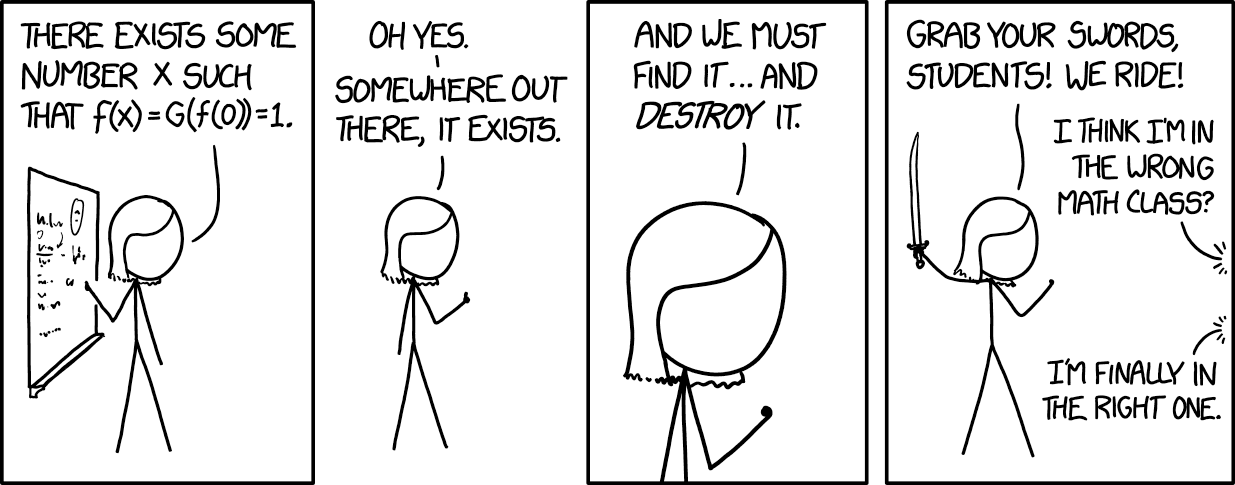
\includegraphics[width=17.15in]{images/existence_proof_2x} \caption{Hopefully you are in the right place. Credit XKCD  [permalink](https://xkcd.com/1856/)}\label{fig:xkcd-preamble}
\end{figure}

\hypertarget{how-many-kinds-of-people-are-there}{%
\chapter{How Many Kinds of People Are There?}\label{how-many-kinds-of-people-are-there}}

\begin{quote}
There are 10 kinds of people in this world.
Those who understand binary code and those who don't.

--- seen on a T-shirt
\end{quote}

\hypertarget{things-are-about-to-get-meta-right-from-the-start}{%
\section*{Things are about to get meta right from the start}\label{things-are-about-to-get-meta-right-from-the-start}}
\addcontentsline{toc}{section}{Things are about to get meta right from the start}

I'm going to start off this first chapter in a book about data science with an unsubstantiated claim. My claim is this: People love to categorize themselves and others. They love to take quizzes online that tell you ``what kind of person you are'' in some way or another. They love to make statements that begin with, ``there are two kinds of people in this world\ldots{}'' and so on. Ok? That's my claim. It's a bit of a mouthful.

Now, I just made a claim in support of which data \emph{can absolutely} be brought to bear. But I won't use data to support it. What? Why not, for cyring out loud?! This is a book about data science!!! The reason is this: this book encourages you to think critically and skeptically about all kinds of ideas, claims, and questions. It tries to show you how to talk about these ideas precisely and not succumb to fallacies and bad intuition. But while trying to develop these skills, it is important to know when we are in turbo critical thinking mode (that's a technical term\footnote{Just kidding; it's not really a technical term.}) and when we're not. Sometimes, we need to be able to say common-sense things and not have to support them.

What \emph{exactly} am I even saying in my claim, you might be thinking? What do you mean by, ``people love to'' do X, where X, like \_\_\_\_\_\_ {[}``blank''{]}, is a stand-in for some of the specific things I mentioned. That everybody does X? Most people? That people who do X derive pleasure above some pleasure threshold, thus designating ``love'' as opposed to ``like?'' You see, I could have tried to make my claim more precise. And I could have found polls and published reports that estimate just how many people have, by choice, taken some kind of person-category-test-thing, or posted funny jokes about ``two kinds of people.'' But I'm just letting my claim stand as a common-sense claim. Just like if I said, people love going to the movies. I wouldn't feel the need to cite a scientific study to support that claim.

Now, if someone is making what to \emph{them} appears to be a common-sense claim but to you appears false or at least non-obvious, you have a few options. You can challenge the assumption and ask for evidence. Or you can accept the assumption, \emph{for argument's sake}, to see where this is going. Hopefully, my claim feels common-sense enough to you too (i.e., we have that in common). If not, I'll just ask you to follow along to see where this is all going\ldots{}

\hypertarget{two-kinds-of-people}{%
\section{Two Kinds of People}\label{two-kinds-of-people}}

\hypertarget{sec:categories}{%
\subsection{Categories, counts, and kinds}\label{sec:categories}}

``There are two kinds of people\ldots{} which one are you?'' questions have become something of an internet meme, particulary with the categorizations represented graphically or pictorially. There is a whole \href{https://2kindsofpeople.tumblr.com/}{blog devoted to them by João Rocha}. The images in Figure \ref{fig:tp-fig} probably need no explanation, as they concern the great \href{https://en.wikipedia.org/wiki/Toilet_paper_orientation}{toilet paper orientation} debate.

\begin{figure}
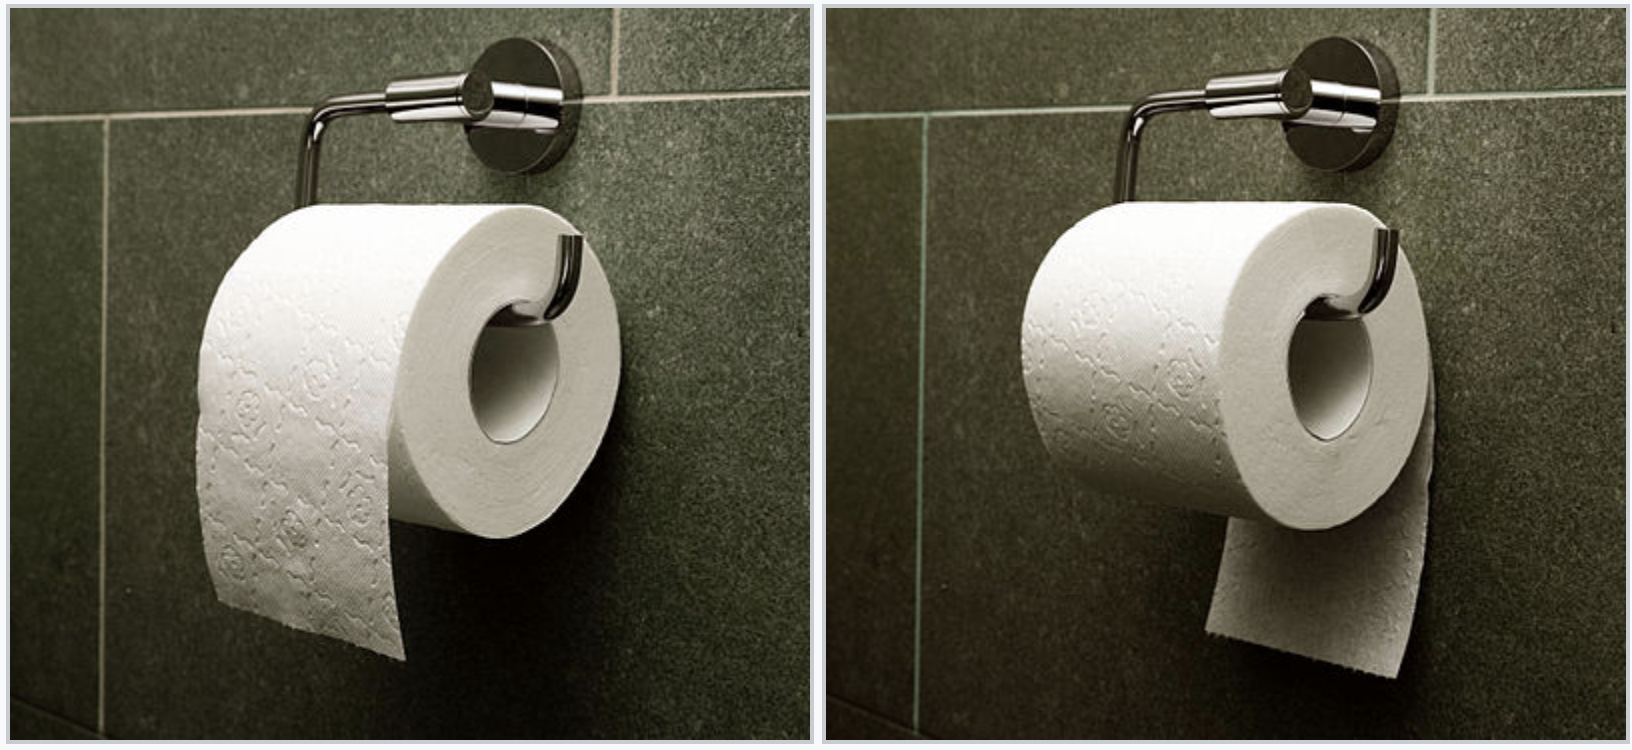
\includegraphics[width=0.9\linewidth]{images/Toilet_paper_orientation_overunder} \caption{The greate debate}\label{fig:tp-fig}
\end{figure}

source \href{https://commons.wikimedia.org/wiki/File:Toilet_paper_orientation_over.jpg}{Wikimedia Commons User:Elya}

Toilet paper orientation is a distinguishing \textbf{test question} that separates people into one of two ``kinds'' (or ``types'' or ``categories''; sometimes English has several words that are used interchangeably). A fancy word for this ``splitting into two'' is dichotomy (die-COT-uh-mee), from the Greek. A \textbf{dichotomous question} has two possible answers. Here, you choose one way to orient the roll or the other. Let's call this roll choice ``over'' (shown on left) or ``under'' (shown on right). Perhaps you have debated which is better with a friend or family member. Or perhaps you are lucky enough to have never thought about it at all. In any case, armed with this particular test question, we can go out and collect some data.

\label{tab:tp-table}How people roll

counts

over

21

under

19

I went ahead and asked 40 people in Washington Square Park in New York City which kind of person they were, and the results are shown in Table \ref{tab:tp-table}. This being a book about data science, you might think I'm going to start calculating proportions right away, for example by saying that 52\% of New Yorkers are over-hangers.
Nope. Although you should be able to figure out that proportion conversion, it is not the point I want to focus on right now.

That point I want to focus on is that, based on our data, there \emph{are} indeed two kinds of people here. If, for example, everyone in the world were an under-hanger (heaven forbid), then I couldn't very well say that there were two kinds of people in this world. At least not with regard to toilet paper orientation. It would be like if I presented you with the data in Table \ref{tab:dumb-table}. Looking at that, I can't very well convince you that there are two kinds of people.

\label{tab:dumb-table}People in Washington Square

count

person

40

not a person

0

That all seems pretty obvious, in part because I made up a \emph{tautology} in the second example there. Being a person is automatically associated with everyone who can be a \emph{kind of person}.

But what if I had gotten exactly the same results for the toilet paper question? What if the data looked like Table \ref{tab:tp-redux}. In this \textbf{alternate universe}, everyone I ask in Washington Square is an under\_hanger. Yes, it's one of those scary alternate universes, like the Twilight Zone. Anyway, does that mean that there is only one kind of person when it comes to toilet paper orientation? Well\ldots{}not necessarily. After all, this was just a \textbf{sample} of people in Washington Square. It was not the whole \textbf{population} of Washington Square, even, let alone New York City, let alone the world.

Go ahead and put a pin in that idea. We'll come back to it later. For example, we might want to know how confident we can be about a larger population from a sample. That's kind of a big thing in statistics.

\label{tab:tp-redux}How people roll (alternate universe)

count

under

40

over

0

\hypertarget{checkpoint}{%
\subsubsection{Checkpoint}\label{checkpoint}}

While focusing on the great toilet paper debate, we've managed to establish some important fundamental ideas.

\begin{itemize}
\item
  Dichotomous questions split people into two kinds, but only as long as it is actually possible for both answers to occur.
\item
  In an alternate universe, people might give different answers than they do in this one. (Seriously, this is an important idea).
\item
  Clearly, we can ask people questions that prompt them to choose between more than two categories. But ``two types of people'' questions are more fun.\footnote{That was another unsubstantiated claim.} I mean there are so many of them! So\ldots{} does that mean that there really are two types of people? To answer this, we will need to get into another great debate.
\end{itemize}

\hypertarget{dimensions}{%
\subsection{Dimensions}\label{dimensions}}

\begin{quote}
``I always said if I had one breakfast to eat before I die, it would be Wonder Bread toasted, with Skippy Super Chunky melted on it, slices of overripe banana and fresh crisp bacon.''

--- \href{https://nypost.com/2008/07/26/mayors-last-meal-is-a-killer/}{Michael Bloomberg}
\end{quote}

Former NYC mayor Michael Bloomberg is a chunky peanut butter kind of person. Are you? As peanut butter comes in ``smooth'' and ``chunky'' varieties (also known as creamy and crunchy, respectively), this question is also a dichotomous one. However, if we add this test question to our question pool, in addition to the one about toilet paper orientation, we will soon find that having two two-kinds-of-people questions begins to imply more than two kinds of people. Wait, what?

See, back when I went to talk to the people in Washington Square, I also asked them about the great peanut butter debate. As you can see from Table \ref{tab:pb-counts}, smooth came out slightly ahead.

\label{tab:pb-counts}How people spread

counts

chunky

17

smooth

23

But this second question did not erase the first question. In fact the first few rows of our data from Washington Square look like this:

\begin{verbatim}
##    roll spread
## 1 under chunky
## 2  over chunky
## 3 under smooth
## 4  over chunky
## 5 under smooth
## 6 under chunky
\end{verbatim}

If we count each combination as it occurs--that is, under-chunky, over-chunky, under-smooth, and over-smooth--we get the results shown in Table \ref{tab:tpxpb}. There are four combinations, because we have two questions with two possibilities (dichotomies) for each. Before you read on, it's a good time to ask yourself if you can answer the following questions (answers in the footnote): (a) if there were two questions with three categories each, how many combinations could be observed? (b) if there were three dichotmous questions, how many combinations could be observed?\footnote{(a) 9, (b) 8}

\label{tab:tpxpb}Two questions

chunky

smooth

over

9

12

under

8

11

Table \ref{tab:tpxpb} is an example of a kind of table that is so common in data science, it has its own name. Three of them, in fact. It is sometimes called a cross table (or crosstab), or a \textbf{two-way table} (makes sense), but most commonly it is known as a \textbf{contingency table} (wha? I'll explain later in Section \ref{sec:indep}.) I'm sorry that there are three names for the same thing. Really I am.

Ok, now things are about to get deep. The title of this chapter is ``How Many Kinds of People are There?'' And we've now explored how using two two-kinds questions leads to four types. You've probably figured out yourself that you take the product (i.e., multiply) of the number of categories in each of the questions, and that tells you how many ``buckets'' you can have overall. But still, there are different ways to arrive at different bucket numbers.

\label{tab:newpb}PB preference

counts

chunky

13

don't care

3

hate all

4

smooth

20

Consider Table \ref{tab:newpb} in contrast to \ref{tab:tpxpb}. We've now given people four choices to express their peanut butter preference. In addition to chunky and smooth, they can also choose to say that they hate all peanut butter or don't care. We now have four kinds of people. But since we make the determination of what kind of person you are using just one (kind of) question, we say that there is one \textbf{dimension} (in this case, peanut butter preference) along which people can be divided into four groups. In Table \ref{tab:tpxpb}, there were two dimensions, a dimension of peanut butter and a dimension of toilet paper. Notice that this word, dimension, is used in much the same way as when we refer to geometric space as being two-dimensional (e.g., a drawing on flat sheet) or three-dimensional (e.g., a solid object, or sometimes a drawing that creates the illusion of looking at a solid object.) The three dimensions of space are often labeled something like (x, y, z). Here, our two dimensions could be labeled (pb, tp). The order doesn't matter. To summarize, in Table \ref{tab:tpxpb}, we have two dimensions and four kinds. In Table \ref{tab:newpb}, we have \emph{one} dimension and four kinds.

So far so good: two questions, two dimension, right? Well\ldots{} maybe. We already saw that if a question does not actually divide people into kinds, because only one answer appears, then it doesn't really count. It is not a dimension. In our contingency table representation, this might look like the left side of Table \ref{tab:tpxpb-alt}. In an alternate universe, no one prefers smooth to chunky. Another way to say it is that the peanut butter question is not \textbf{informative}.

\label{tab:tpxpb-alt}Two questions (alternate universes)

chunky

smooth

over

21

0

under

19

0

chunky

smooth

over

0

21

under

19

0

But now consider the alternate universe on the right of Table \ref{tab:tpxpb-alt}. In that case, everyone who is an over-hanger of toilet paper prefers smooth peanut butter, and everyone who is an under-hanger prefers chunky. If this is the case, there are only two kinds of people, at least in our sample. Those who over-hang \emph{and} prefer smooth and those who under-hang \emph{and} prefer chunky. But does it make sense to say there are two dimensions? We did ask two different questions!

You might reason about it the following way: in our sample, if I ask anyone just one of the two questions--about either toilet paper or peanut butter--then I immediately know the answer they would give to the other one. I don't actually have to ask two questions, other than to establish in the first place that I didn't have to. Since I only get information from one question, there is only one dimenion.

If I could play a gong sound right now, I would. Wait a minute. At least \emph{you} can if you are reading this book in a web browser. Go for it:

\href{http://soundbible.com/2148-Chinese-Gong.html}{source}

\hypertarget{sec:indep}{%
\subsection{Independence, Association, and Contingency}\label{sec:indep}}

\begin{quote}
This section title sounds like a philosophy book by the late Richard Rorty.
--- inner voice
\end{quote}

We just spent a little bit of time in an alternate universe, a bizarro world in which knowing how someone prefers to orient their toilet paper tells you what style of peanut butter they like, and \emph{vice versa}. Notice that this knowing-about relationship is symmetric, and that in fact, the two representations as shown in Table \ref{tab:tpxpb-alt2way} are informationally equivalent.

\label{tab:tpxpb-alt2way}Alternate universe (two equivalent ways)

chunky

smooth

over

0

21

under

19

0

over

under

chunky

0

19

smooth

21

0

In our regular universe, however, this relationship was not observed. In Table \ref{tab:tpxpb}, all four possible combinations occur. When knowledge about a person's answer to one question provides information about their answer to another question, we say that the two answers are \textbf{contingent} upon one another. This is the reason we called the two-way table a contingency table in the first place, although it is still called that even when two answers are not contingent. Go figure. Contingent is another word for \textbf{dependent}. To make matters worse, we \emph{also} often say that the two responses are \textbf{associated}.

In our bizarro world scenario, one answer completely determines the other. This \textbf{deterministic} relationship is one extreme in the spectrum of association/dependence/contingency. At the other extreme, if the two responses are not at all associated/dependent/contingent, then we say that they are \textbf{independent}. To say that two responses are independent is to assert that knowing one of them does not give you any information about what the other one might be. This would have been my intuition, at least, about toilet paper and peanut butter. But whether they are independent or mildly associated with one another is an empirical question, which means we should try to answer it with data. In bizarro world, where they were deterministically related, we might reasonably want to know why. Could there a gene that turns on toilet paper orientation and peanut butter preference at the same time?

\hypertarget{sec:factors}{%
\subsection{Latent Factors and Measurement}\label{sec:factors}}

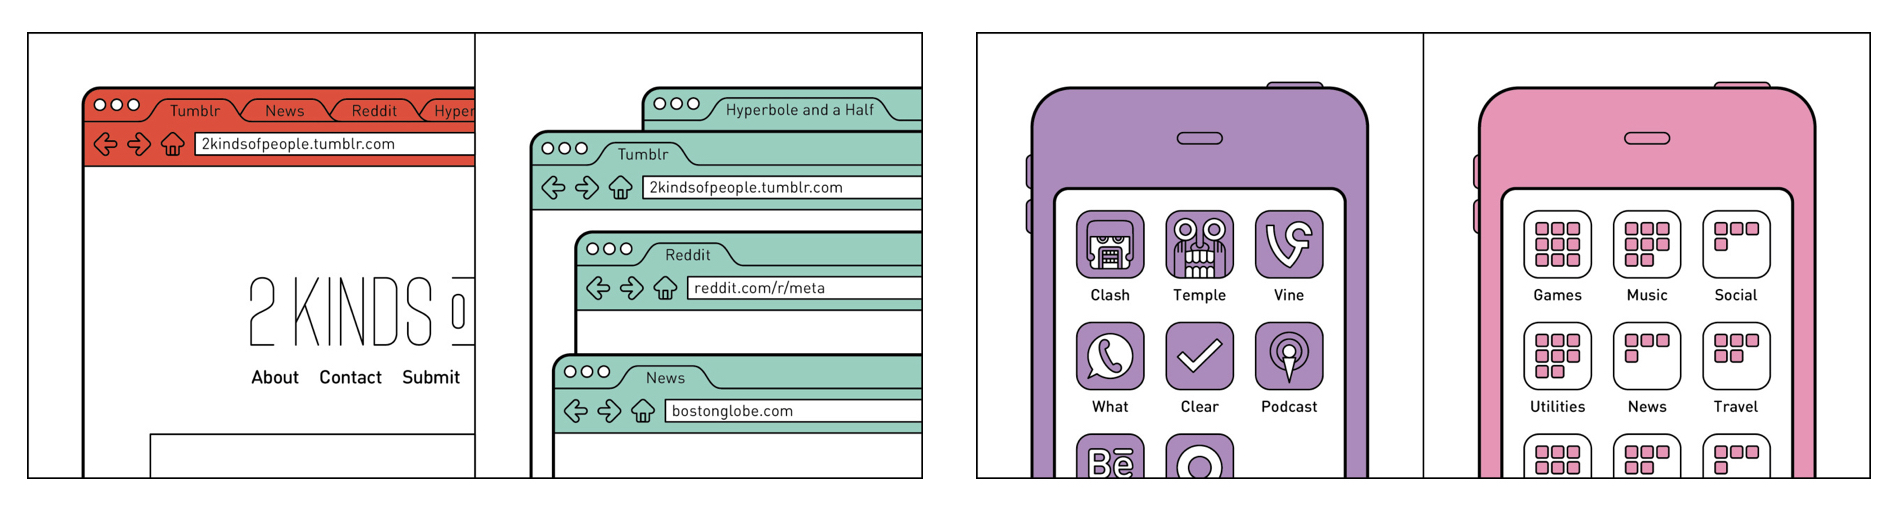
\includegraphics{images/two-two-kinds.jpg}
\href{https://2kindsofpeople.tumblr.com/}{source}

Figure \ref{fig:apps-windows} shows two more two-kinds of people graphics from João Rocha's blog. I bet that you can identify yourself with one of the two images in each pair. I certainly can. But ask yourself, given our discussion above, do you think the choices a person would identify in each case above are independent or not independent (e.g., contingent, associated, dependent)?

In contrast to the toilet paper and peanut butter questions, which at least appear to be about totally different things, these two dichotomies have something similar going on in each of them. The choice on the left is about organizing your desktop browser, either in tabs or as separate windows. The choice on the right is about organizing apps in your smartphone, either loose or in folders. We might say that both of them get at a tendency to organize your digital environment. Call it digitidness (short for digital tidiness). This tendency, we may imagine, might even carry over into non-digital environments, like your actual desk, bookshelf, or filing cabinet.

What we've done here is to try to explain the association between responses to the two questions (assuming that there is, i.e.~that they are not independent) by appeal to some underlying \textbf{latent factor}. We say a factor is latent (meaning hidden) because we don't observe digitidiness itself directly, but we only observe tidy browsers or smartphone app folders. Perhaps you can think of another candidate factor besides digitidiness. In any case, we might propose that each of the two two-kinds questions in Figure \ref{fig:apps-windows} are in fact indirect \textbf{measurements} of the same factor. If so, this could explain why the two answers woudl be associated.

\begin{quote}
Notice that a \textbf{factor} is also a dimension, in the sense we used before. We could have said ``latent dimension'', but we tend to use the word factor when we are drawing attention to the specific nature of the dimension rather than just counting. We also sometimes use the word \textbf{trait}. At least in psychology, trait tends to be reserved for stable psychological factors. Thus ``stress'' can be a factor but not a trait, whereas ``social anxiety'' may be a trait, if it is persistent. In this case, digitidiness might be considered a trait (and thus also a factor and a dimension).
\end{quote}

Contrast this with toilet roll orientation, which we can observe directly just by looking in someone's bathroom. (We assume that they are telling the truth when they answered our questions, but we could in principle verify it.) It was only in the bizarro world when toilet roll orientation and peanut butter preference were perfectly related that we started to wonder if there maybe \emph{was} an underlying genetic factor. Genetic factors were once not directly observable either, but we assumed them for explanatory value. Today we can of course observe specific genetic variation, although there are still many gaps in our understanding of the relationship between genes and observed behaviors.

Consider some data again, in two possible worlds, shown in Table \ref{tab:tabsxapps}. On the left, we have the deterministic scenario we saw before. As before, we identified this situation as having two kinds of people and really just one dimension. In contrast to before, where we had no real explanation for this coincidence, we attribute it now to some factor, like digital tidiness.

\label{tab:tabsxapps}Possible data for digital tidiness

folders

loose

tabs

21

0

windows

0

19

folders

loose

tabs

16

6

windows

5

13

But now consider the possible results in the table on the right. Since all four possible quadrants have non-zero counts, we see that knowing whether someone organizes their browser using tabs does not completely (i.e., \emph{deterministically}) specify whether or not they put their apps into folders. On the other hand, one answer \emph{does seem to be associated} with the other. Notice that the values are still much higher in the ``buckets'' that we think of as indicating the presence or absence of digitial tidiness. These are the tabs-folders bucket (tidy) or the windows-loose bucket (not tidy). We say that the tidiness factor appears to explain much of the observed range, or \textbf{variance}, in responses to the two questions. But it doesn't explain all of it, since there are people (11 out of 40, in this case) who don't fall into one of these buckets.

This situation on the right is probably more realistic. After all, very few things in this world are absolute (unlike in bizarro world). So now the big question re-emerges: are there two kinds of people or four? One dimension, or two? It's sort of\ldots{}like\ldots{}in between\ldots{}?

It might be gong time again:

\textbf{Golda says}: Although digitidiness explains a lot of what we see in our data, it doesn't explain it all. I believe that desktop tidiness and mobile tidiness are different, if related, tendencies For example, when we use mobile phones, we're typically on-the-go and have less time. If we knew more about the people in our sample, we might see that these discrepancies in the organization of apps and tabs actually relate to other aspects of their lives. So, I say there are two dimensions.

\textbf{Sidney says}: Digitidiness is the only real factor here, but people may not always be consistent in these particular behaviors. Also some people are only sort-of-tidy, and apply this tidiness unevenly but randomly. These two-kinds of people choices don't leave room for shades of gray, so that's what we're seeing in the mixed categories where people are tidy in one environment and not in another. But ultimately there is really just one dimension here.

\textbf{What do you think?}

\hypertarget{shades}{%
\subsection{(An Infinite Number of) Shades of Gray (or Brown)}\label{shades}}

We've taken the two-kinds-of-people idea pretty far in this chapter already. But it's time to acknowledge the elephant in the room. Not every question about attributes, preferences, or behaviors can be answered in such an either/or manner. Digitidiness might be one of those things. Consider the following dialogue:

\begin{quote}
Stacy: ``There are liberal and conservative kinds of people, Trang. Which one are you?''
Trang: ``Well, you know I'm not sure I'm exactly one or the other. I think I'm somewhere in the middle.''
\end{quote}

Although we often use them as \textbf{discrete categories}, the words liberal and conservative might be better thought of as endpoints of \textbf{continuous scale}. In fact, they might even apply to different \emph{dimensions} of political thought with respect to social issues or economic issues. If you think about it, it's not hard to come up with other examples of ``categories'' that really just describe one end or another of a continuous scale. Yes, there are short people and tall people, but everyone has a height, and a lot of people are ``about average.'' Height is just a number on some scale. So it wouldn't necessarily make sense to put people into the categories of tall or short.

In the great toilet paper debate, we were able to identify two kinds of people based on two possible responses to the question of roll orientation. Two answers; two kinds. If instead of discrete categories, we have a number on a continuous scale, does that mean that there can't be ``kinds'' of people anymore? To answer this question, we'll need to understand what exactly we're talking about when we characterize people using a continuous scale.

Consider poopiness. Some people are really poopy (close to poopiness = 1), some aren't poopy at all (close to 0), and most are somewhere near the middle of the scale. That's not a very quantitative description. I used the words ``some'' and ``most'', but I didn't give you counts like I did in Table \ref{tab:tp-table} about toilet roll orientation. If I showed you the poopiness data for sample of people, the list would look something like this.

\label{tab:unnamed-chunk-7}Don't ask me how I got these numbers.

poopiness

0027

0.679

0083

0.473

0015

0.703

0024

0.691

0029

0.495

0014

0.833

Poopiness is a number, and these data are called \textbf{numerical} or \textbf{quantitative} as opposed to \textbf{categorical}. It's not as easy to make sense of a bunch of decimal values like this as it is to look at simple counts of categories. However, this problem has been solved by using dot plots, stacked dot plots, and histograms, which you can read all about in any standard textbook, for example OpenIntro Statistics, Chapter 2. I'm going to go straight into the histogram, which most likely you've seen before. It's the most commonly used representation for data of this kind.

\begin{figure}
\centering
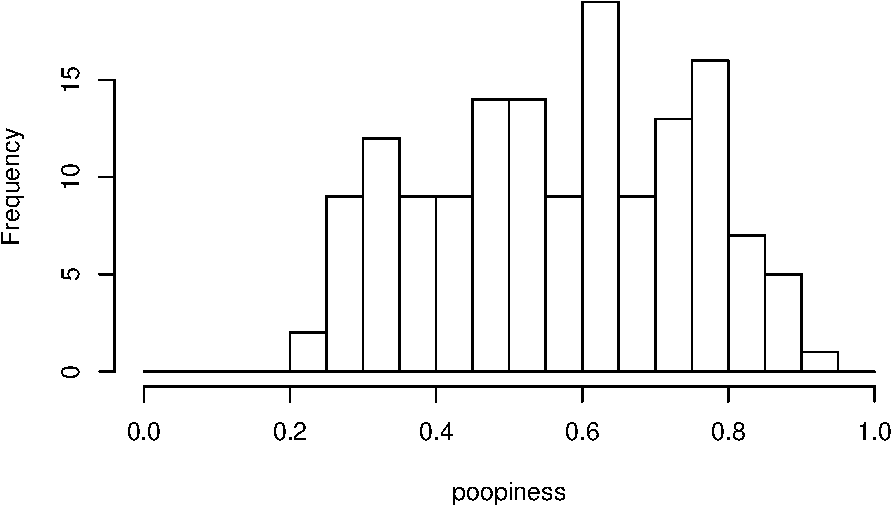
\includegraphics{bigquestions-book_files/figure-latex/poopy-hist-1.pdf}
\caption{\label{fig:poopy-hist}Histogram of Poopiness}
\end{figure}

A histogram is a bar plot of counts for poopiness values that fall into certain numerical ranges.
Consider the range of poopiness values from 0.4-0.45. Our data set has 9 values in this range, so the height of the bar above this range on the x-axis is 9.\footnote{Technically, this range is a semi-open interval, (0.4,0.45{]}, so that any values exactly equal to 0.45 can only be included in one bin and not the ones on either side.} The y-axis in Figure \ref{fig:poopy-hist} is labeled ``frequency'', which is just another word for counts. Some more jargon: the ranges are called ``bins'' and the numerical values that separate the bins are called ``breaks.'' In Figure \ref{fig:poopy-hist}, the breaks are at increments of 0.05 (e.g., 0, 0.05, 0.1, 0.15, 0.2, 0.25, \ldots{}).

\begin{quote}
Question: Given that there are 20 possible bins in the histogram in Figure \ref{fig:poopy-hist}, but only 15 of them have non-zero counts, are there 20 kinds of people (in terms of poopiness) or 15 kinds of people?
\end{quote}

Trick question? You bet. The breaks (and thus bins) in a histogram are arbitrary. I can choose any breaks I want, as long as all of the data points fall into exactly one bin. (I can't just exclude some bins, though. That would be cheating.) The histograms in Figure \ref{fig:poopy-hist-alt} are both perfectly valid histograms. One of them has four bins, and one of them has only two bins.

\begin{figure}
\centering
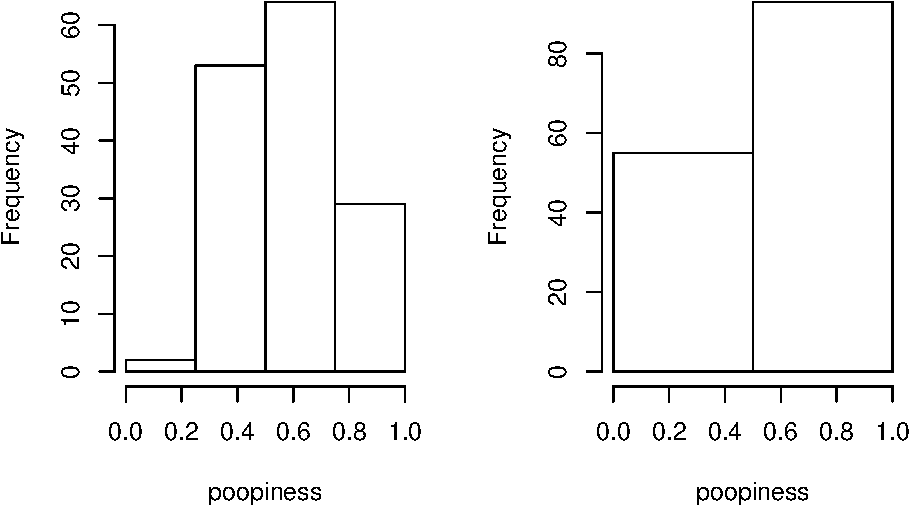
\includegraphics{bigquestions-book_files/figure-latex/poopy-hist-alt-1.pdf}
\caption{\label{fig:poopy-hist-alt}Other Histograms of Poopiness}
\end{figure}

It's tempting to take the counts on the right of Figure \ref{fig:poopy-hist-alt} and declare that there are two kinds of people. After all, this gets us back to familiar territory. Ta-dah!

\begin{figure}
\centering
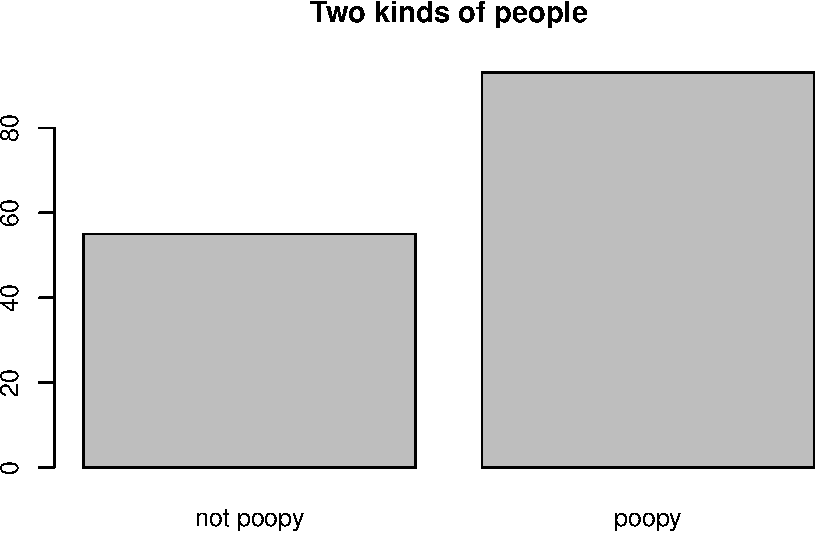
\includegraphics{bigquestions-book_files/figure-latex/poopy-two-kinds-1.pdf}
\caption{\label{fig:poopy-two-kinds}This is terrible, horrible, no-good, very-bad thing to do.}
\end{figure}

As you can tell, because it says so right in the figure caption, this is terrible, horrible, no-good, very-bad thing to do. Why is it a bad thing to do?

\begin{enumerate}
\def\labelenumi{\alph{enumi})}
\tightlist
\item
  The split was made at 0.5 on the poopiness scale, but that is not the average value of poopiness in the data set, which is closer to 0.57, as can be seen is Figure \ref{fig:poopy-hist} (or from the ``raw'' data themselves).
\item
  You should always use at least 5 bins when you have numerical data
\item
  Representations of data should communicate honestly about the nature of the data themselves. In this case, poopiness is not a category.
\end{enumerate}

What I did here was take a numerical/quantitative value (poopiness) and mis-represent it as a categorical value. I did it by \emph{dichotomizing} it, i.e., by splitting off everyone above 0.5 and labeling them as ``poopy''. I could have alternately split at the mean or median value and labeled the resulting two groups as ``low poopiness'' and ``high poopiness.'' But this would still have been a mis-representation. It would hide the fact that poopiness comes in a continuous range of values.

\begin{quote}
ASIDE (\emph{delivered in a hushed voice}): I won't be able to convince you of this now, but it turns out that if you do this---if you dichotomize numerical data---you will BREAK STATISTICS! Ok, that sounds a bit dramatic. But in all seriousness, one of the jobs of statistics is to understand associations between different variables, such as poopiness and, say, earning potential. If you treat poopiness (or other variables) as discrete when they are really continuous, you may very well get the wrong answers. As the man down the street from where I used to live often muttered to himself while waving his arms in the air, THAT IS AN ABSOLUTE IRONCLAD MATHEMATICAL FACT. No, but in all seriousness, there is a terrific paper on exactly this subject \citep{maccallum2002}.
\end{quote}

Dang it! you say. You've taken me down this rabbit hole of poopiness for too long. How many kinds of people are there? Are you saying that if one looks at properties that are described by numbers instead of categories, that there is only one kind of person? Is it all just shades of gray (or brown)?

\hypertarget{mixtures}{%
\subsection{Mixtures}\label{mixtures}}

Remember Figure \ref{fig:poopy-hist}? (Don't click it!) Here it is again so you don't have to scroll back. Data scientists like to say this picture shows you the \textbf{distribution} of poopiness in our sample. Statisticians use the word distribution in a more formal way that is best put off until we actually need it. We don't need it yet.

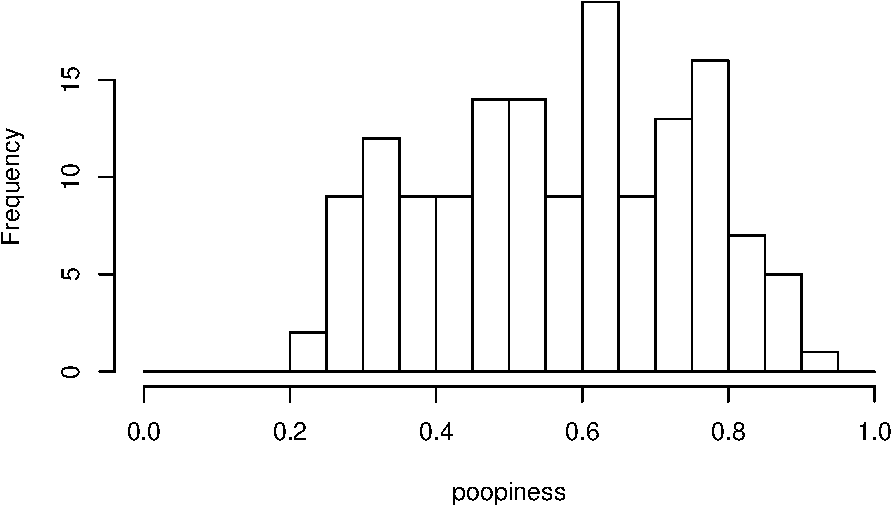
\includegraphics{bigquestions-book_files/figure-latex/poopy-hist2-1.pdf}

What if I told you that there ARE two kinds of people; you just can't see them unless I give you special glasses (or more information). If I gave you special glasses (or information), you would see this:

\begin{figure}
\centering
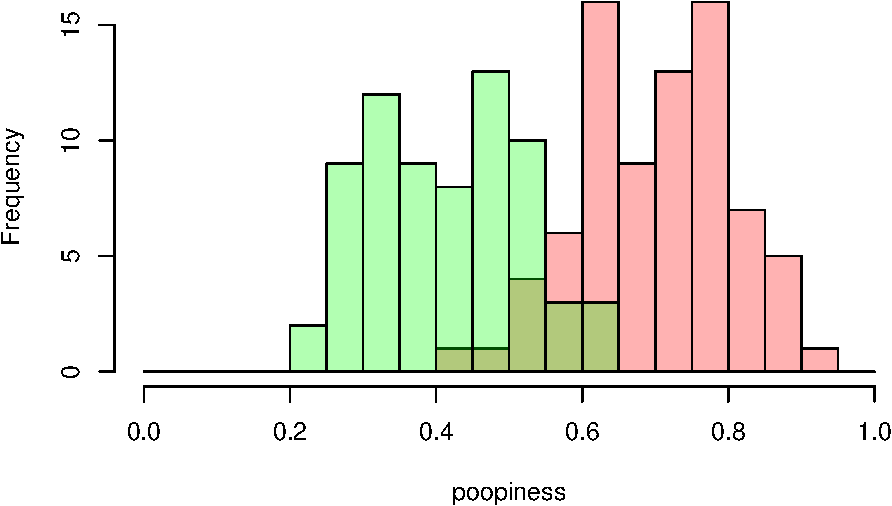
\includegraphics{bigquestions-book_files/figure-latex/poopy-hist-mixture-1.pdf}
\caption{\label{fig:poopy-hist-mixture}A mixture of poopiness}
\end{figure}

\emph{By what dark magic have you colorized the data!} you say. Or, perhaps you just said, hm, interesting.
In Figure \ref{fig:poopy-hist-mixture}, I've made a histogram with bars in two different colors, light green and pink. The colors are slightly transparent so that you can see both the green and pink distributions in their entirety even though they overlap. That's what the brownish bars mean. You're looking at the overlap of the green and pink bars, not another set of bars. Now, if you compare this histogram closely with the original, colorless histogram above, you'll see that the bin ranges are the same (width=0.05), and the the counts of green and pink bars add up to the total values that we had before. If there are green people and pink people, or in any case two different kinds of people, and if their poopiness is distributed as shown in Figure \ref{fig:poopy-hist-mixture}, then the poopiness of the mixture of these two groups of people will look just like Figure \ref{fig:poopy-hist}.

Ok, but that doesn't explain how you would know that there are two groups. If I didn't tell you. That's because \emph{you wouldn't necessarily know. You would need to have more information}. Now you might suspect something if you saw a distribution that looked like this:

\begin{figure}
\centering
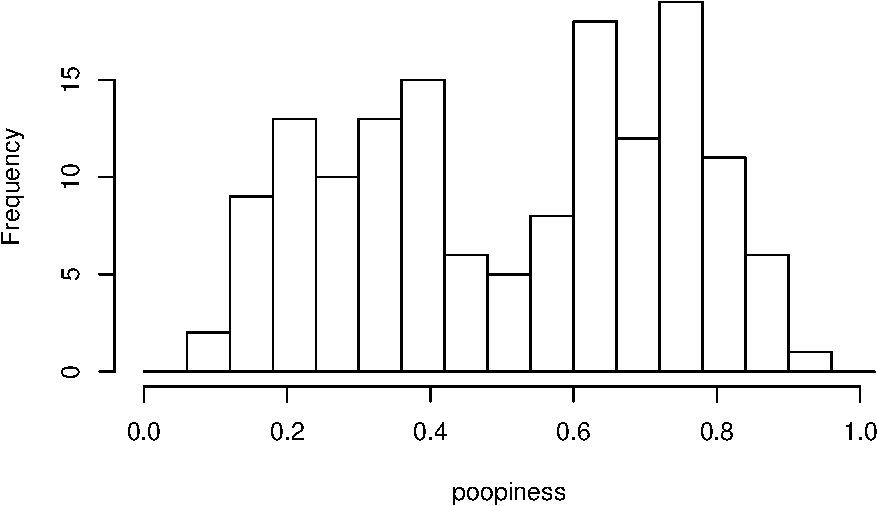
\includegraphics{bigquestions-book_files/figure-latex/poopy-hist-mixture-suspicious-1.pdf}
\caption{\label{fig:poopy-hist-mixture-suspicious}A suspicious mixture of poopiness}
\end{figure}

In Figure \ref{fig:poopy-hist-mixture-suspicious}, the distribution has a double-hump like a Bactrian camel. In spite of that, it is not called a Bactrian distribution--which would make me happy--but a \textbf{bimodal} distribution. The point that I'm trying to make here is that a bimodal distribution makes you suspect that there could actually be two groups mixed together in our data.

But the original data for poopiness did not look bimodal. I suggested to you that you would need more information to determine if there are two groups. And so, I present you with\ldots{} Crappiness! For each of the subjects in our poopiness data set, we have also collected data on their crappiness. Crappiness is also a numerical value ranging from {[}0,1{]}. It's sort of like poopiness, but different. Here are some values:

\begin{verbatim}
##      poopiness crappiness
## 0027     0.679      0.453
## 0083     0.473      0.627
## 0015     0.703      0.159
## 0024     0.691      0.519
## 0029     0.495      0.806
## 0014     0.833      0.147
\end{verbatim}

And here\ldots{}(drum roll please)\ldots{} is a histogram of crappiness!

\begin{figure}
\centering
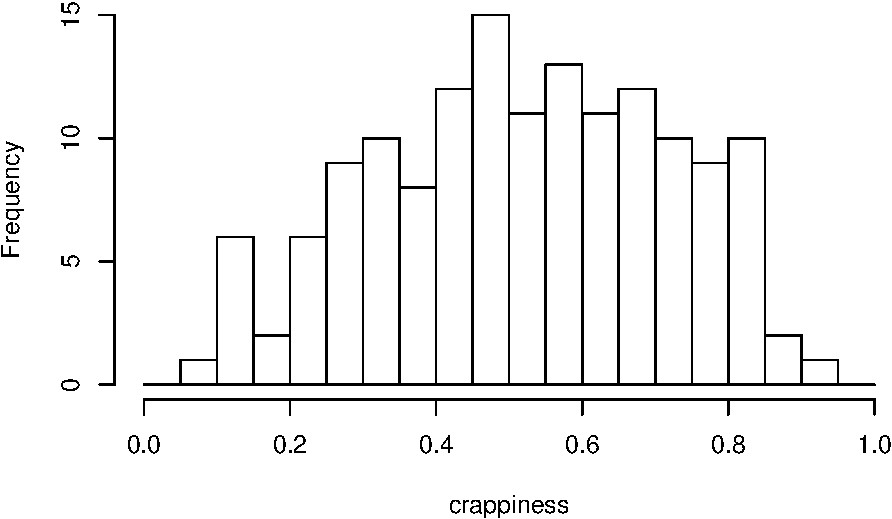
\includegraphics{bigquestions-book_files/figure-latex/crappy-hist-1.pdf}
\caption{\label{fig:crappy-hist}Histogram of Crappiness}
\end{figure}

Hmm. I bet you were hoping that the crappiness data would look obviously bimodal, but it's not obvious. Nevertheless, hopefully you trust that I wouldn't lead you on a wild goose chase for no reason. Perhaps you can even see it coming. If we look at poopiness and crappiness separately, there is no clue that there might be distinct groups of people in our data set. But if we look at them together\ldots{} there is.

When we looked at categorical data for two two-kinds-of-people questions, we made 2x2 contingency tables. We also used the word ``dimension'', for example to say that we were describing people along two dimensions (recall: toilet paper and peanut butter). Now that we are looking at numerical data (poopiness and crappiness), we can also use two dimensions, as in a two-dimensional scatterplot, to examine both variables at once. This scatterplot is shown in Figure \ref{fig:poopy-crappy}. Each point represents data from one person, with their poopiness value on the x-axis and crappiness on the y-axis.

\begin{figure}
\centering
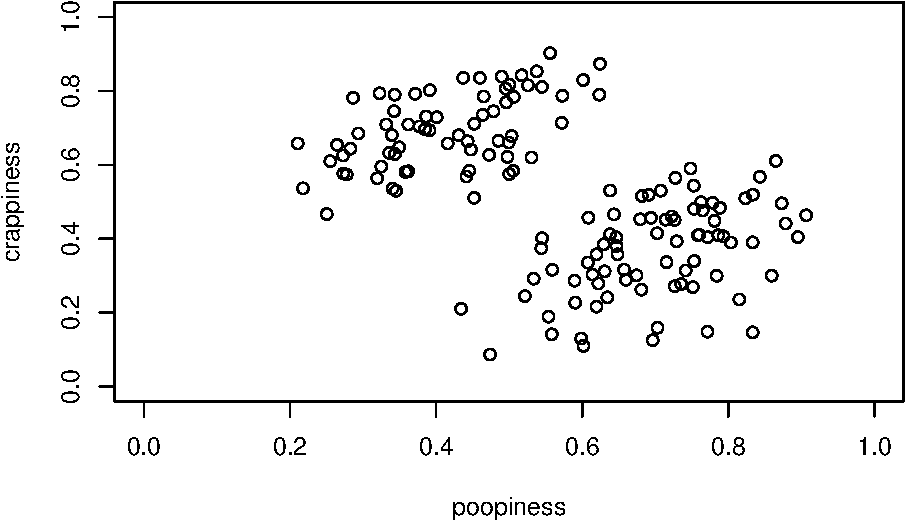
\includegraphics{bigquestions-book_files/figure-latex/poopy-crappy-1.pdf}
\caption{\label{fig:poopy-crappy}Scatterplot of Crappiness vs Poopiness}
\end{figure}

Alas, oh data! Your bimodal nature has revealed itself in the higher-dimensional plane!

How many kinds of people are there? When it comes to poopiness and crappiness, people exhibit a continuous range of values, so we can't neatly put them into buckets. Neither poopiness nor crappiness appear to be bimodally distributed on their own. However, when examined together, as in the scatterplot in Figure \ref{fig:poopy-crappy}, a pretty suggestive pattern emerges in the data. There are two \textbf{clusters} of points, one group of which is lower in poopiness but higher in crappiness than the other. Interestingly, though, in both groups poopiness and crappiness tend to increase together. That is, they appear to be associated, not independent.

I do not mean to imply that clusters of points can always be found if we have data along many dimensions. That is certainly not always the case. The present example was concocted (I admit it!) to show that groups \emph{can} emerge, even in numerical data. Cluster analysis \citep{kaufman2009} refers to set of data-science methods all about looking for the existence of groups in multidimensional data.

\hypertarget{check-your-understanding}{%
\subsubsection*{Check your understanding}\label{check-your-understanding}}
\addcontentsline{toc}{subsubsection}{Check your understanding}

\begin{enumerate}
\def\labelenumi{\arabic{enumi})}
\tightlist
\item
  Based on the scatterplot in Figure \ref{fig:poopy-crappy} and the grouped-by-color histogram for poopiness in Figure \ref{fig:poopy-hist-mixture}, describe what the equivalent grouped-by-color histogram for crappiness would look like. Would it look the same or different? Explain.
\end{enumerate}

\hypertarget{cut-scores-and-abnormality}{%
\subsection{Cut Scores and Abnormality}\label{cut-scores-and-abnormality}}

\begin{quote}
Because that's not what normal people do.
--- things my spouse says
\end{quote}

If you read the aside in Section @ref\{sec:shades\}, you'll recall that I warned against possible negative consequences of setting arbitrary cut points to dichotomize a data set---that is, turning numerical data on a continuous scale into two categories by using a cutoff value. But now consider the following scenarios:

\begin{enumerate}
\def\labelenumi{\arabic{enumi})}
\item
  To pass the written test for your a driving learner's permit in California, you must answer at least 38 questions correctly out of 46. That's 82.6\% correct. At 80.4\% (37/46) or below, you fail and have to retake the test on another day.
\item
  A patient's blood test shows levels of ALT (alanine aminotransferase) at 77 units per liter. The lab report labels this as ``abnormally'' high, and the physician is concerned about possible liver damage or disease.
\end{enumerate}

These two examples involve just the kind of dichotomization that I cautioned against, and yet they occur very commonly in practice. So what gives? Is it wrong to use cutoffs this way? Why do people do it?

The short answer is that we often find ourselves in need of a classification (pass or fail; diagnose liver disease or not) but without a perfect classification device. Rather we have only indirect measurements (of knowledge or liver function) in some quantitative measure. Perhaps you once found yourself on the ``border'' between letter grades for a course and were particularly perturbed (or relieved) by the imperfections of such a system. Or you may have found yourself with ``slightly'' abnormal levels in a blood test and wondered whether you should seek further tests.

Both the California department of motor vehicles and the physician in our scenarios need to make a decision based on imperfect evidence. They want to be able to say that the person's test results show that they are ready to get behind the wheel of a car, in one scenario, or suffering from liver problems in the other. But all they can really do is express this belief using a \textbf{probability}. This probabilistic judgement is based on a mathematical \textbf{model} that relates traits like readiness-to-drive or liver-disease to certain test results. Understanding how these models come into existence is one of the learning objectives of this course.

The term \textbf{normal distribution} arose in statistics because the particular bell-shaped distribution occurs so frequently. If poopiness were normally distributed in our sample from before it might like this.

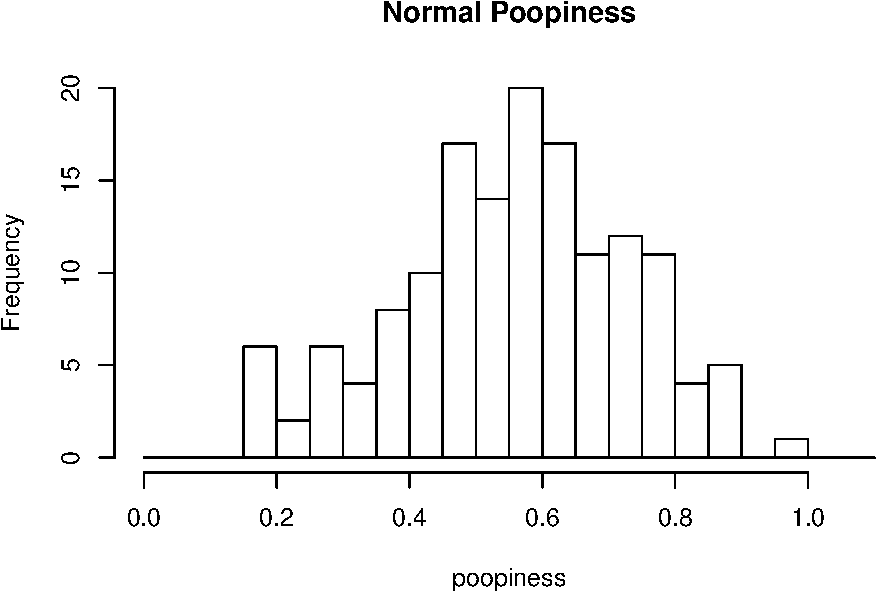
\includegraphics{bigquestions-book_files/figure-latex/normal-poopy-1.pdf}
Technically speaking, all of the values, including the maximal value of 0.962 that we observe in Figure \ref{fig:normal-poopy} are normal. Poopiness varies in the population. It is impossible to be abnormally poopy, under the circumstances. By definition. some values at the extreme ends of a normal distibution are less likely to occur than values in the middle. But still they may occur rarely. It is only when extreme values (large or small) are associated with other conditions of interest, such as the relationship between elevated ALT and liver disease, that it makes sense to ``flag'' these extreme values.

\hypertarget{summary}{%
\subsection*{Summary}\label{summary}}
\addcontentsline{toc}{subsection}{Summary}

\hypertarget{vocabulary}{%
\subsubsection*{Vocabulary}\label{vocabulary}}
\addcontentsline{toc}{subsubsection}{Vocabulary}

\begin{itemize}
\tightlist
\item
  kind, type, category
\item
  dichotomous
\item
  crosstab, two-way table, contingency table
\item
  association, contingency, dependence
\item
  latent factor, dimension, trait
\item
  measurement, model, bimodal, cluster
\end{itemize}

We started out this chapter on a quest to answer our first big question: How many kinds of people are there? En route, we have examined both categorical data, such as from two-kinds-of-people questions, and numerical values like poopiness. The toilet paper and peanut butter orientation questions may seem silly and inconsequential to you. I can only imagine what you might think of the poopiness and crappiness dimensions that I completely made up (I admitted it!). However, in the next section, we will see that when it comes to personality psychology, there are real-world analogues of the discrete/categorical and continous/numerical multi-dimensional descriptions of people that we just saw.

\hypertarget{sixteen-personalities-or-five-factors}{%
\section{Sixteen Personalities or Five Factors ?}\label{sixteen-personalities-or-five-factors}}

Before you read this section, you might want to go ahead and take one of the personality tests based on
the Meyers-Briggs Type Indicator (MBTI) categories and/or the five-factor model of personality (also called the Big Five). There is only one ``official'' MBTI, which is a commercial product. However, there are several free alternatives online which use the same typology classification. There are also several variations of

\begin{quote}
Test yourself:

\begin{itemize}
\item
  MBTI-style at \url{16personalities.com} or \href{https://openpsychometrics.org/tests/OEJTS/}{here}
\item
  Big Five \href{http://www.personal.psu.edu/~j5j/IPIP/}{here} or \href{https://bigfive-test.com/}{here} or \href{https://openpsychometrics.org/tests/IPIP-BFFM/}{here}. \href{https://ipip.ori.org/}{General information about these test items.}
\end{itemize}
\end{quote}

I will only minimially describe the MBTI and the Five Factor Model (FFM, or Big Five) here, in terms of the topics we have been discussing. There are many resources for learning more about these personality tests. Some are referenced under further reading.

\hypertarget{mbti}{%
\subsection{MBTI}\label{mbti}}

The MBTI will categorize people, based on their responses, dichotomously along each of four dimensions, also called ``scales.'' These are:

\begin{itemize}
\tightlist
\item
  Extraversion-Introversion (E-I)
\item
  Sensation-Intutition (S-N)
\item
  Thinking-Feeling (T-F)
\item
  Judging-Perceiving (J-P)
\end{itemize}

Thus there are sixteen possible combinations, for example ``INTP''. Each person is assigned to one of these sixteen personalities. Many online tests will provide you with a report to help interpret your classification. That is, the four dimensions are understood to come together in some holistic picture of your ``type.''

\hypertarget{big-five}{%
\subsection{Big Five}\label{big-five}}

The term ``Big Five'' is a commonly used term for the five-factor model of personality. Based on responses to questionnaires, people are assigned a numerical score along five dimensions (also called scales or factors!)

\begin{itemize}
\tightlist
\item
  Neuroticism refers to the tendency to experience negative feelings.
\item
  Extraversion is marked by pronounced engagement with the external world.
\item
  Openness to Experience describes a dimension of cognitive style that distinguishes imaginative, creative people from down-to-earth, conventional people.
\item
  Agreeableness reflects individual differences in concern with cooperation and social harmony. Agreeable individuals value getting along with others.
\item
  Conscientiousness concerns the way in which we control, regulate, and direct our impulses.
\end{itemize}

\begin{quote}
Fun fact: both OCEAN and CANOE are mnemonic devices that can help you recall the names of the Big Five dimensions.
\end{quote}

Since the results of a Big Five test, such as the IPIP-NEO, are five numbers, you don't get assigned a personality ``type'' by these tests. Rather, you may be provided with an explanation of what it means to score high (or low) on, say, Extraversion. You may have noticed that extraversion (occasionally spelled ``extroversion'') appears on both the MBTI and the Big Five.

\hypertarget{twenty-questions-about-extraversion}{%
\subsection{Twenty Questions (about Extraversion)}\label{twenty-questions-about-extraversion}}

Suppose, for whatever reason, we want to identify a person's extraversion. We may want either (a) to classify them as extraverted or not (i.e., introverted), or (b) to quantify a degree of extraversion, say on a scale of 0-100. Why not then just pose the question in the following way. In the first case:

\begin{enumerate}
\def\labelenumi{\alph{enumi})}
\tightlist
\item
  Choose the one that describes you: Extraverted ~~~~\textbar{} ~~~~Introverted
\end{enumerate}

or, in the second case,

\begin{enumerate}
\def\labelenumi{\alph{enumi})}
\setcounter{enumi}{1}
\tightlist
\item
  Identify yourself on the following scale: Extraversion 0 -- + -- + -- + -- + -- 50 -- + -- + -- + -- + -- 100
\end{enumerate}

Personality tests, such as those we've discussed above, do not ask questions like these. Rather, they include many different questions, sometimes twenty or even more, about things like going to parties, making friends, and drawing attention to oneself.

Why ask twenty questions instead of just one? Recall from the great toilet paper debate (Section \ref{sec:categories}) that no one ever felt it was necessary to ask twenty questions to know whether you were an over-hanger or an under-hanger. However, when we discussed digitidiness (Section \ref{sec:factors}), we suspected that two different questions may have both been getting at the same latent factor. The situation here, in the real-life domain of personality testing, is similar.

Psychologists \sout{believe that extraversion is an underlying factor} invented the idea of extraversion to explain patterns of behavior, including patterns of responses to questions about how people feel in various situations. Such as enjoyment or lack thereof in being the center of attention. The use of indirect evidence such as questionnaire responses to make inferences about psychological traits is the main task of \textbf{psychological measurement} or psychometrics. The main challenge of psychometrics, perhaps even the reason for its existence, is that human beings are noisy.

Put another way, you cannot expect a deterministic relationships between how a person feels or acts in one situation and how they act in another. An extraverted person is not \emph{always} extraverted. And an extraverted person might not always answer questions about their feelings in the same way. It is hard to observe or even self-report on extraversion directly, because extraversions manifests itself differently at different times and in different contexts. Whether this noise is due to some mysterious internal process, like a coin flip in your brain, or due to many unnaccountable external factors, like whether you slept poorly that day, we can't say. What we can say is that human noisiness manifests itself as \textbf{measurement error}.\footnote{The word \textbf{error} makes it sounds like there is a right answer, and that tests get it wrong. This is, indeed, one view. However, you don't have to believe that there is a right answer. For example, you can believe that human beings have some amount of inherent unpredictability.} We can also say that, in spite of measurement error, some patterns do remain.

\hypertarget{but-whats-the-point}{%
\subsection{But what's the point?}\label{but-whats-the-point}}

Trying to describe people in terms of kinds or numerical scales is complicated. Why do we even bother? It's tempting to say that we just want to understand ourselves better, and that is certainly a reasonable answer. Sometimes, though, we want to predict how someone will act in the future, perhaps in a situation that differs from one that they have faced in the past. In that case, we can't exactly use the past to predict the future, unless we do so by making inferences about underlying traits from past behaviors and then predicting how someone with those particular traits would act in a new context. This purpose drives some uses of tests based on the MBTI and the Big Five, for example by employers or career counselors. However, although the MBTI is oftern used for these purposes, one should exercise caution in doing so \citep{pittenger1993}. You should certainly not assume that all personality tests do an equally good job of providing information for the desired inferences.

According to the standards of the American Psychological Association \citep{american1999}, whenever psychological tests are used for some specific purpose (e.g., employment, admission to a school or hospital, or even in court) there must be a valid argument for the intended purpose of the test scores. This \textbf{validation argument} will usually involve many facets, including how consistent the results of the test are, whether it is a fair test for all groups of people, whether test scores really are associated with relevant outcomes in the domain of use, and so on. These arguments, and challenges to them, are all part of validity.

\hypertarget{still-meta-after-all-these-pages}{%
\section*{Still meta after all these pages}\label{still-meta-after-all-these-pages}}
\addcontentsline{toc}{section}{Still meta after all these pages}

I'd like to point out that we still haven't even once asked a question of the form ``what proportion of people\ldots{}'' or ``what is the probability that a person\ldots{}?'' There's nothing wrong with these questions, and we will have plenty of time to investigate questions of this kind in the remaining chapters about other Big Questions. But to be true to our question about how many kinds of people are there, we didn't need to know all of the specifics. Our discussion has been rather \emph{metaphysical}, in the sense that we have tried to understand how differences that we observe among people can be expressed in terms of kinds (categories) or numbers, which are different \emph{kinds} of data. Whoa.

\hypertarget{exercises}{%
\section*{Exercises}\label{exercises}}
\addcontentsline{toc}{section}{Exercises}

\hypertarget{when-and-how-will-you-die}{%
\chapter{When and How Will You Die?}\label{when-and-how-will-you-die}}

\begin{quote}
It is difficult to make predictions, especially about the future.

--- Niels Bohr (probably)
\end{quote}

In our first Big Question, we began to look at individual differences between people or what statisticians call variation within a population. If there is no variation---like in the bizarro world where everyone orients their toilet paper in the ``under'' orientation---then there is nothing to talk about, at least not statistically speaking. There is, however, considerable variation in health outcomes and human lifespan. Lots to talk about there. In our next Big Question, we ask ``when and how will you die?'' and ``what, if anything, can you do about it?''

What kind of question is, ``when and how will you die?'' Well, according to some of my colleagues, it's a morbid question. Feelings aside, we might say that it sounds like a prediction question, since it's about the future. So to explore this big question, we will need to understand what it means in general to make a forecast about some future event. We'll also find it useful to distinguish between predictions that are or are not explanatory. Most efforts in health sciences attempt to explain relationships between behavioral and genetic factors and health outcomes. In particular, they try to understand causal effects. So in this module, we will try to understand causal explanations more generally.

\hypertarget{not-quite-death-but-um-rain}{%
\section{Not Quite Death, but, um\ldots{} Rain?}\label{not-quite-death-but-um-rain}}

Perhaps its a good idea to warm up, before we face the grim reaper. What does it mean to say there's a 30\% chance of rain tomorrow in New York? Does it mean that it will definitely rain in 30\% of the city (say, Brooklyn), but not in the other 30\%? Or that it will rain for 30\% of the day (say, from 8am-3pm). Here are some possibilities to consider:

\begin{enumerate}
\def\labelenumi{\alph{enumi})}
\tightlist
\item
  It will definitely rain in some parts of the city but not in all of them
\item
  It will definitely rain for some part of the day in all of the city
\item
  It will definitely rain for some part of the day in some of the city
\item
  It may or may not rain anywhere in the city at any point in the day.
\end{enumerate}

Read here for an \href{http://wxbrad.com/why-a-50-chance-of-rain-usually-means-a-100-chance-of-confusion/}{explanation of what meteorologists \emph{probably} mean}

\hypertarget{stochastic-vs-deterministic-variables}{%
\subsection{Stochastic vs Deterministic variables}\label{stochastic-vs-deterministic-variables}}

Sometimes when I say definitely, I mean probably. Like if I say, I'm definitely going to do something about all of this clutter on my desk. But when I really mean business, I say deterministically. It definitely sounds more serious.

Meteorologists---scientists who model the weather---cannot tell us deterministically about weather events. A \textbf{deterministic} description of an event would be something like, if I let go of the umbrella I am holding in my hand, it will fall to the ground. If A then B. No exceptions. Weather events are \textbf{stochastic}. They have an element of randomness, like tossing a coin or rolling a die. So, just as we can say that a coin has a 50\% chance of coming up heads---assuming it is a fair coin---we can make statements like there is a 30\% chance that it will rain tomorrow.

\hypertarget{ensembles}{%
\subsection{Ensembles}\label{ensembles}}

One way to think about the 30\% chance of rain is to imagine that our experience in the world is one possibility in a multiplicity of possible worlds. See, I told you this idea of multiple universes was going to be important! Imagine that there are 10 possible worlds indistinguishable from ours, and that tomorrow it will in fact rain in 3 of them. The key idea is that we don't know which one of these possible worlds is the one we are actually experiencing\ldots{}

There is another way to think of 30\%. Suppose a meteorologist told you, I'm 30\% sure it is going to rain tomorrow. This time, 30\% represents a degree of belief. Importantly, the degree of belief is subjective. Here it is attributed to a meteorologist, which might make you take it more seriously than if your Uncle Bob said the same thing (unless Uncle Bob is actually a meteorologist). Anyway, degree of belief is subjective. Which doesn't mean it's arbitrary or just a matter of opinion. When it comes to forecasts, some people or some forecasting models are going to be right more often than others. More on that later.

In the meantime, if we take this forecast of rain seriously, we have decisions to make. It could be whether or not to take an umbrella with us when we leave the house tomorrow, or whether to cancel our plans to have a barbecue outside. These decisions may not seem very high stakes. The worst case scenario is that we get wet. But other decisions we have to make on a daily basis can have more serious consequences for our health or even our life. We often have to make those decisions based on {[}partial, subjective, probabilistic{]} information\ldots{}

\hypertarget{death}{%
\section{Death}\label{death}}

I highly recommend this data visualization from Flowing Data called \href{https://flowingdata.com/2015/09/23/years-you-have-left-to-live-probably/}{Years You Have Left to Live, Probably}

Here is a screenshot, although it's not nearly as interesting when you can't interact with the simulation and watch the little balls drop.

\begin{figure}
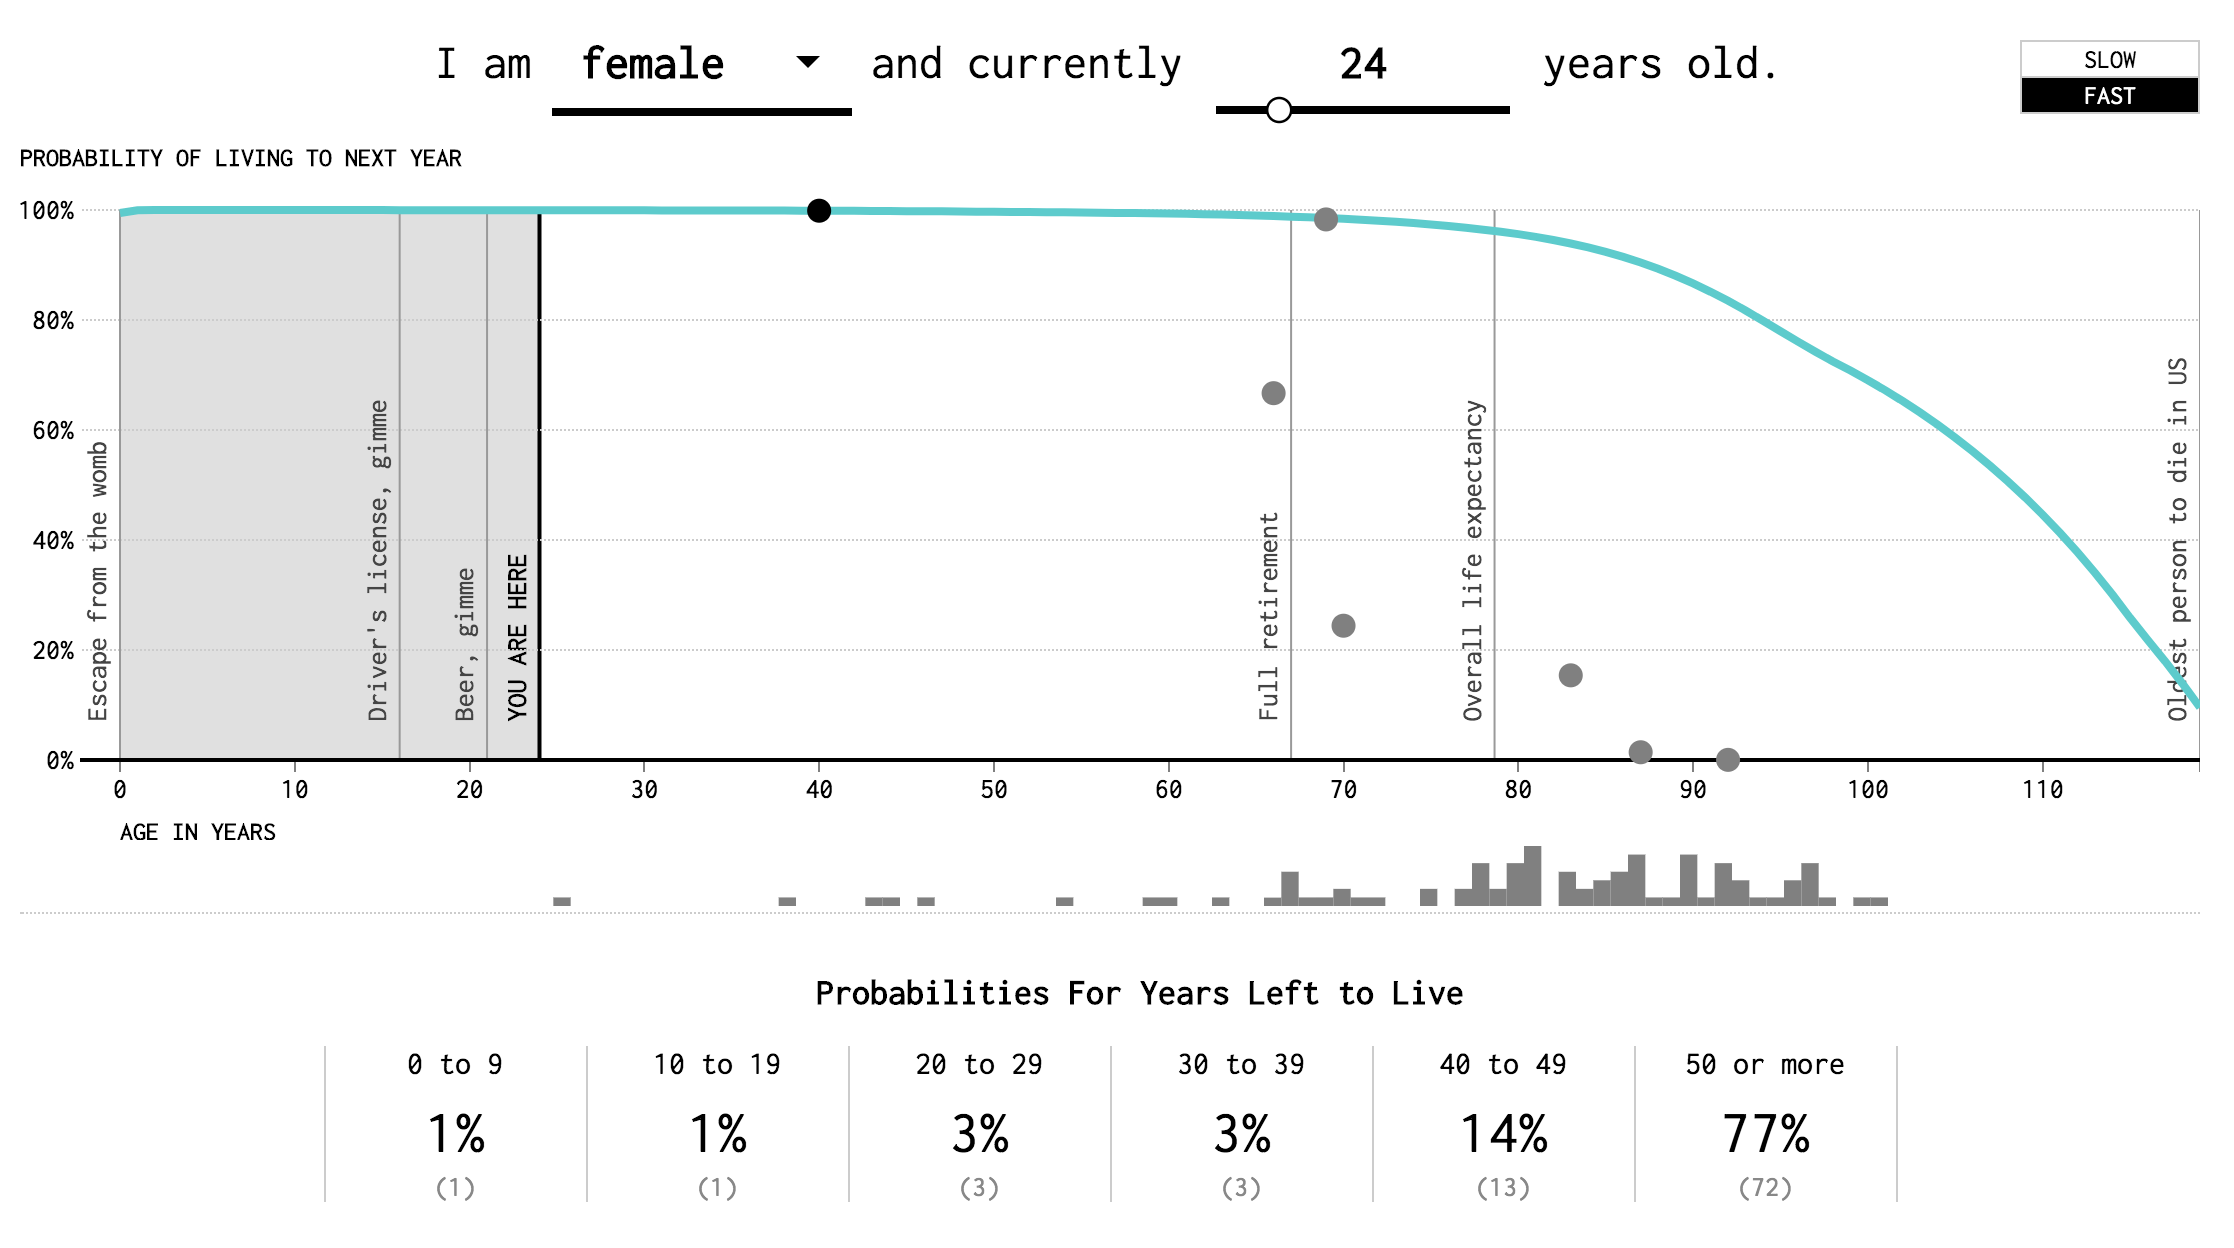
\includegraphics[width=0.9\linewidth]{images/YYHLTLScreenshot1} \caption{Screenshot of interactive data visualization}\label{fig:years-screen}
\end{figure}

\hypertarget{conditional-probabilities}{%
\section{Conditional Probabilities}\label{conditional-probabilities}}

\hypertarget{bayes-rule-with-disease}{%
\section{Bayes Rule with disease}\label{bayes-rule-with-disease}}

\hypertarget{causality}{%
\section{Causality}\label{causality}}

Does eating meat cause heart disease? Does smoking cause lung cancer? What does it mean to say A causes B? First of all, this may sound like a philosophical question, and indeed the philosopher David Hume shed some important light on the question of how we conceive of causation. But this is a course on probabilistic thinking, not philosophy. So we are going to take a more pragmatic approach and focus on how we use the concept of causation in everyday life. Nevertheless, it helps to first recall our distinction between deterministic and stochastic processes. If I hit a porcelain tea cup hard with hammer and the tea cup breaks, we can safely say that hitting the teacup with a hammer caused the cup to break. We don't really feel the need to say that if you hit a teacup hard with a hammer, there is a 99.9997\% chance that it will break. Even if that's actually true. And we don't feel the need to define ``hard'' in this case either. We use an example like a teacup and hammer when we want to focus on the big picture and not the details. And the big picture here says that hitting a teacup with a hammer deterministically causes the teacup to break. If we don't hit In the case of the physics of hammers and teacups, we feel that we know this much is true.

What about buying a lottery ticket? Does buying a lottery ticket cause one to win the lottery? Well, you certainly are not guaranteed to win the lottery if you buy a ticket. In fact, your chances will be very low. But you can't possibly win if you don't buy a ticket. So, strictly speaking, buying a ticket or not does influence the probability of buying a ticket.

We've now seen two examples

In the first case (hammer and teacup):
If A (hammer hits teacup) then definitely B (teacup breaks)
If not A (hammer does not hit teacup) then definitely not B (teacup does not breaks)

Teacup breaks
Teacup doesn't break
Hammer hits teacup
Always\emph{
Never
Hammer does not hit teacup
Never}
Always
*pretty much; we're not splitting hairs here.

In the second case (lottery ticket):
If A (buy lottery ticket) then maybe B (win lottery) and maybe not B (do not win lottery)
If not A (do not buy lottery ticket) then definitely not B (do not win lottery)

Now, let's pause for a moment and think about the question we started with: does smoking cause cancer? Does it fit either of these two cases?

Unfortunately the question about smoking does not. It belongs to a yet another case.

In the third case (smoking):
If A (smoke) then maybe B (cancer) and maybe not B (no cancer)
If not A (do not smoke) then maybe B (cancer) and maybe not B (no cancer)

Now we're not saying that the chances of cancer are the same whether you smoke or not. That remains an open question so far as our present argument goes. But even thus far, we can see that the smoking causality question, posed this way, invites some more questions.
How big a difference does there have to be between the cancer rates for smokers and non-smokers for us to be convinced that there is an association between smoking and cancer?
After all, there are a lot of other factors including behavior and genetic factors
Why do we believe that the association between smoking and cancer is a causal relationship (specifically, smoking causes cancer)?

\hypertarget{will-you-make-money}{%
\chapter{Will You Make Money?}\label{will-you-make-money}}

\begin{quote}
No one can win at roulette unless he steals money from the table while the croupier isn't looking.

--- Albert Einstein (possibly)
\end{quote}

The development of probability theory is historically linked to attempts to understand games of chance, especially ones in which money was involved (see for example, \href{http://sites.math.rutgers.edu/~cherlin/History/Papers2000/cheng.html}{here}. Sometimes betting money on an uncertain outcome falls under the name of gambling; other times it's dignified with the name investment or ``smart business decision.'' But regardless of the label, there are smarter and less smart ways to play money games.

\hypertarget{battle-of-the-bills}{%
\section*{Battle of the Bills}\label{battle-of-the-bills}}
\addcontentsline{toc}{section}{Battle of the Bills}

Let's recall a distinction we made earlier in this course about deterministic and stochastic or random processes. This time, we'll think about two different bets you make with your friend. In the first bet, you and your friend are debating whether it was Bill Paxton or Bill Pullman in the movie Apollo 13. To make the game interesting, you bet two dollars. You look it up on the internet, and find that it was indeed Paxton. One of you wins. Do you feel the need to check again? Probably not. This particular question, although you may not have known the answer for sure, has only one possible answer.

Now consider another bet, this time for three bucks! You and your friend are walking down the street debating the ``merits'' of mint chocolate chip vs.~cookies and cream as ice cream flavors. You claim that mint chocolate chip is the more popular flavor, and decide to ask the first passer-by which flavor they think is better. Suppose they don't just ignore you, thinking you're a nutcase, and they answer cookies and cream. Are you satisfied with this one answer? Or do you feel the need to ask another pedestrian? And how many?

We might say that the variable ``BPA'', which stands for ``which Bill P. starred in Apollo 13?'' has a deterministic answer, but the variable ``MCCoCAC,'' which stands for ``mint chocolate chip \textgreater{} cookies and cream?'' can take on one of two answers (no ties allowed) depending on whom we ask. Because it is a random or stochastic variable, we have to talk about it using different terms. We might say something like, what proportion of people (in this neighborhood, say) prefer cookies and cream? Or what are the chances that the first person we ask will express that particular preference.

This may all sound like silly bets that are really just games between friends. But people make small and large money bets all the time, in everything from business and life decisions, to recreational games. In this chapter, we explore probability calculations that inform things like advertising, airplane booking, the job market, and march madness.

\includegraphics{bigquestions-book_files/figure-latex/unnamed-chunk-10-1.pdf}

Consider the diagram on page 83 of the Naked Statistics chapter that you read at the beginning of this module. This diagram shows the drug approval process from investment to pay off. At each node of the graph, there are two possibilities: first, you may or may not develop a drug that cures a particular disease. Next, even if the drug works, it may or may not get approved. And even if it gets approved, it may or may not make it to the market. At each branch, there are two possibilities with estimated probabilities (note: how do we estimate these probabilities in practice?). All of the branches lead to 5 possible outcomes, with different pay-offs. Using what we know about all of the possibilities, all of their probabilities, and the potential payoffs, we can estimate what is called ``expected value''. {[}walk through expected value calculation{]}. This value represents the average amount of money we would expect to make, if we invested in a lot of drugs, that all went through this same process independently.

Question to think about: even though the expected average pay-off is \$4,225,000, which is more than 4 times the original investment, would you want to make this investment for any single drug? Why or why not?

Now that we've made this calculation empirically, it might be helpful to simulate it in R! \url{https://a3sr.shinyapps.io/Drug}

Week 9 Video 1
Let's now return to the example that you read about last week (Wheelan, chapter 5):
In 1981, Schlitz brewing company, now defunct but at one time the largest beer producer in the US, ran a bold advertising campaign. During the Super Bowl, Schlitz ran a live blind taste test against one of its competitors, Michelob. 100 Michelob drinkers participated in the taste test, which aired LIVE. The advertisement slot itself cost a lot of money. Schlitz could have just run a funny ad involving puppies on the beach, so why take a risk with a taste test that could conceivably have gone badly. How could Schlitz have been so confident that their beer would be preferred?

THINK ABOUT IT QUESTION: What information would you need to know to advise the Schlitz brewing company about running such an ad? (please take a few minutes before continuing on, to try to list this information on your own).

As discussed in the book, some things we would need to know are:
Intended sample size for taste test
Actual proportion of Michelob drinkers who would prefer Schlitz in a blind taste test
Acceptable outcome of live taste test for promoting Schlitz beer
Rules of mathematical probability

Run and discuss simulation in Shiny: \url{https://a3sr.shinyapps.io/Schlitz/}
Week 10 Reading 1
In the last two weeks, we've explored the concept of expected value. As you may have noticed, expected value can be very useful for making decisions, but it does not tell the whole story. In the college majors example, expected career earnings for each possible major were only useful in describing what happens on average, for a lot of people going through the job market. However, we still had a lot of uncertainty about what would happen to any single individual who pursued a career in acting or accounting. Similarly, we would not have been as confident running the Schlitz commercial with a sample of 10.

This brings us to one of the most important concepts in probability and statistics: the ``law of large numbers''. Random variables are by definition, random, so we cannot predict any single outcome -- we can only say how often we expect a particular outcome to occur if we observe a lot of data. Thus, you might see how expected value is particularly useful in situations where the same process gets repeated many times. In the airplane overbooking example, there may be a reasonable probability that airlines will lose money on any given flight. But airlines can make probability calculations to ensure that they earn money than they lose overall.

The usefulness of the law of large numbers is particularly evident in gambling. Many people go to casinos and play the same games over and over again, which each (theoretically) have consistent probabilities of winning or losing. One person may win and another may lose, but if a lot of people play a game of roulette (for example), casinos can estimate approximately what proportion will win and how many will lose. And, the more games that are played, the more confident the casino can be about their predicted proportion of wins/losses.

As you've probably heard, casinos are designed such that the house always has the advantage. In other words, every casino game is designed such that the casino always has a slightly better chance at winning than the player. That doesn't mean that players can't win individual games, it just means that, assuming enough people play the game, the casino will almost surely win more games than all the individual players.

This construct tempts us to believe that we can cheat the system. There is a long and interesting history of people trying to figure out betting strategies that will give them back the advantage. The Martingale betting strategy is one example. Please read the following article to learn more about it! \url{https://www.roulettesites.org/strategies/martingale/}

Week 10 Reading 2
As a final example of how we can use probabilistic thinking to inform betting decisions, let's consider March Madness. March Madness is a basketball tournament, where 64 teams compete. In the first round, 32 games are played. The winners of those games then play each other in the 16 second round games. This continues until a single team is named victorious. Every year, people make bets on which teams they think will win each match-up. Data from regular season games can be used to estimate the probability of any team winning a particular match-up, and this information is readily available to fans. Yet, despite the wealth of data that is available to make game predictions, no one has ever correctly predicted all of the sequential game winners in the tournament. In fact, only one person has ever predicted the first two rounds perfectly (this happened in 2019!). How is this possible? In order to learn more about the complexities of choosing a March Madness bracket, please read the following article: \url{https://www.scientificamerican.com/article/how-much-math-do-you-need-to-win-your-march-madness-pool/}

Week 10 Video 1
Now that you know a little more about March Madness, let's just consider the probability of predicting the entire first round correctly. To start, we will (incorrectly) assume that every team has a 50\% chance of winning their first round game. In this case, we have a 50\% chance of guessing the correct winning team. Given that there are 32 games in the first round, how could we calculate the probability of predicting them all correctly? {[}walk through calculation, drawing a tree diagram, similar to those in the first two weeks of the module{]}

\hypertarget{is-the-system-stacked-against-you}{%
\chapter{Is the System Stacked Against You?}\label{is-the-system-stacked-against-you}}

At this point in the course, you've seen how variance in outcomes can be understood in terms of random, or noisy, statistical processes. If you bet on red at the roulette table five times in a row, and if you lose five times, that doesn't mean the roulette wheel isn't fair. That just could be bad luck (for you; possibly good luck for someone else who betted on black). Of course, the casino odds are stacked against you in the long run, since the casino always has an edge. For example, bets on red or black have even odds, but there are two out of 38 possible roulette outcomes in which neither black nor red will win. Now, in principle everyone knows that this is how casinos work, and indeed why they are able to stay in business. So if you end up losing more often than you win in a casino, you can only blame yourself.

Sometimes, though, outcomes are distributed in a certain way that causes us to question whether everything is indeed working as it is supposed to be, at least according to the rules of probability. In particular, when outcomes differ for some group or groups of people, we sometimes worry if the system is fair. You may have heard people say, the system isn't fair.
Well, sometimes it isn't, we might be able to identify an issue problem and even fix it. For this to work, though, we need to understand what outcomes are fair outcomes, and this turns out to be a complicated issue!

Let's start with a simple example, though, to remind ourselves about sampling and differences. We'll walk through this example very naively on purposes. Suppose we take 100 NBA basketball players as a sample and a 100 NYU graduate students as another sample, and now we look at the distribution of heights in each of our samples. We'll look at male graduate students, since the NBA players are also males {[}show actual data here{]}. I don't think any of you are surprised to see that there is a big difference here; that NBA players are, on average, 10 inches taller in fact. If someone asked you, what are the chances of a difference in samples like this occuring by chance, you can actually calculate an answer to that question. Food for thought: What would you need to know as inputs to that estimation?

Pause the video to think about the question and pick an answer:
Which of the following would you need to estimate the chances of the difference in height occuring by chance?
Group sample means
Group sample variances
Sample size of groups
1 \& 2 only
2 \& 3 only
1 \& 3 only
1, 2, \& 3

Now, suppose we accept that NBA players are systematically taller. Could it be that the NBA makes people taller? Perhaps there is special practice or vitamin supplements that NBA players use that causes them to grow 10 inches? Well, we could rule this out if, for example, we examined the heights of NBA players just BEFORE they became NBA players. If we did that, we would see that they were already tall. Now, of course we knew this, but again, it's informative to reason through this simple example as though we didn't necessarily know. Another possibility, then, is that NBA players are selected for their being tall. Okay, let's suppose we convince ourselves that it is true. The question we might now ask, though, is: is that fair? We're saying that short people have a low likelihood of being hired as NBA players. (Note that we're not suggesting that being tall is sufficient to become an NBA player, but it does seem to be necessary). What do you think? Pause the video again to respond to the following:

Which of these statements do you most agree with?
It is not fair; everyone should have an equal chance to play in the NBA
It is not fair; shorter people, who are otherwise talented in basketball, should have an equal chance to play in the NBA
It is fair; tall players perform better because their height provides an advantage in the game of basketball
It is fair; tall players look better on the court than short players
It is neither fair nor unfair; it just is.

While I'm not saying it isn't possible to defend different answers to this particular question of fairness, most of us agree that professional sports are by design selective on performance. In a game like basketball, height provides an advantage which, along with athleticism, makes a player perform better. We might even draw this set of claims this way:

Athleticism →
Height → Performance → NBA

Week 11 Video 2
It makes sense that players in the NBA would be selected for height, since height impacts performance in basketball. So professional basketball players are more likely to be tall. What if I told you that professional hockey players are more likely to be\ldots{}.born in the first three months of the calendar year. What? Yes, you heard that right.

Okay, let's work through this idea similarly to the way we did when sampling from the NBA.
But first, we need to know: in which months are babies born\ldots{}
\url{https://www.cdc.gov/nchs/fastats/births.htm}

Let's take a look at this table of births by month in the United States from 2017. Let's concentrate on the number of births alone and in particular on the first four months of the year, January, Feb, March, and April. Pause the video to consider the following question:

What do you think is the most plausible explanation for the variation in the the number of births in each of these four months
There is chance variation is any random process, such as childbirth
Odd numbered months are more likely to have higher birth numbers
Births are likely to go up and down in month-long cycles
The number of days in each of the first four months of 2017* is 31, 28, 31, 30
(*) Not a leap year
Answer key:
While true, the size of the variation between these months is much too large to be explained by chance alone. Sample size is key here! Indeed if January and February were each equally likely, and we observed only 600 births in total instead of 600,000, then the chance of observing 313 or more births in one month or the other is actually about 27\%. That is, there's about a 13.5\% chance or January having more than 313 births and a 13.5\% chance of it having fewer than 287 births (the rest going to February). However, even if we just up the sample to 6000, the chance of observing more than 3130 births in one month or the other goes down to about 0.05\%, while for 600,000 births, the chances of a discrepancy this large is a number so small it has no meaningful interpretation. So, in short, chance alone can't explain it.

No, you probably guessed that the length of each month explains most of this effect. But not ALL of it. If every day of the year were equally likely, we can estimate the number of expected births using 3855500/365 = 10563. How many births would we expect in a month that had 30 days? {[}pause{]} Well, for months with 31 days, we would expect 31*10563 = 327453 births (rounding), for months with 28 days, 295764. Notice that the difference is large. Notice also, though, that it's larger than the observed difference, and that each of the observed monthly birth counts are lower than expected. That must mean that some months get MORE births. And indeed this is true. Just look at July-October

So, we've established that there are more births in the third quarter of the year (July-Sep) than in the first quarter (Jan-Mar). Now that we've had a chance to think about what we might expect if there is no bias in birthday months of professional hockey players, it's time to investigate this in a little more detail.

Resource: \url{https://journals.plos.org/plosone/article?id=10.1371/journal.pone.0057753}

\bibliography{book.bib,packages.bib}


\end{document}
